\section{Lineární regrese. Užití v deskriptivních, kauzálních a prediktivních úlohách, volba modelu, vlastnosti odhadů}

\subsection{Základní myšlenka}

Lineární regrese je model, kterým popisujeme vztah mezi závisle proměnnou $y$ a jednou nebo více
vysvětlujícími proměnnými $x_1,\ldots,x_k$. Základní populační model má tvar:
\[
y_i = \beta_0 + \beta_1x_{i1} + \cdots + \beta_kx_{ik} + u_i.
\]

V maticovém zápisu:
\[
y = X\beta + u.
\]

Kde:
\begin{itemize}
    \item $y_i$ je hodnota závisle proměnné u pozorování $i$,
    \item $x_{ij}$ je hodnota $j$-té vysvětlující proměnné u pozorování $i$,
    \item $\beta_0$ je konstanta,
    \item $\beta_j$ je regresní koeficient,
    \item $u_i$ je chyba modelu, tedy vše, co ovlivňuje $y_i$, ale není zachyceno v proměnných $x$.
\end{itemize}

Lineární regrese modeluje podmíněnou střední hodnotu:
\[
\mathrm{E}(y_i|x_i)=x_i^\top\beta.
\]

To znamená, že model neříká, že všechny body leží přesně na přímce nebo rovině. Říká pouze, že
\emph{průměrná očekávaná hodnota} $y$ při daných hodnotách $x$ je lineární funkcí vysvětlujících proměnných.

\subsection{Interpretace koeficientů}

Koeficient $\beta_j$ říká, o kolik se změní očekávaná hodnota $y$, pokud se $x_j$ zvýší o jednu jednotku
a všechny ostatní vysvětlující proměnné zůstanou stejné:
\[
\frac{\partial \mathrm{E}(y|x)}{\partial x_j}=\beta_j.
\]

Toto je tzv. \textit{ceteris paribus} interpretace.

\paragraph{Příklad.}
Pokud odhadneme model:
\[
\widehat{price} = 500000 - 2 \cdot km,
\]
pak koeficient $-2$ znamená, že auto s o 1 km vyšším nájezdem má v průměru o 2 Kč nižší cenu.
Pokud je $km$ v tisících kilometrů, znamená to pokles ceny o 2000 Kč při zvýšení nájezdu o 1000 km.

\paragraph{Důležité.}
Samotná regrese ještě neznamená kauzalitu. To, že auta s vyšším nájezdem mají nižší cenu, neznamená
automaticky, že každý další kilometr přesně způsobí stejný pokles ceny. Může jít jen o popis vztahu v datech.

\subsection{Deskriptivní, prediktivní a kauzální použití}

\subsubsection{Deskriptivní použití}

Cílem je popsat vztah mezi proměnnými. Ptáme se například:
\[
\text{Jak se v datech mění cena auta s počtem najetých kilometrů?}
\]

V deskriptivní úloze nám jde hlavně o shrnutí vztahu v datech. Nemusíme nutně tvrdit, že jde o příčinný
efekt.

\subsubsection{Prediktivní použití}

Cílem je co nejpřesněji predikovat nové hodnoty:
\[
\hat y_0 = x_0^\top \hat\beta.
\]

U predikce je méně důležité, zda má každý koeficient přesnou kauzální interpretaci. Důležité je, zda model
dobře predikuje nové hodnoty, ideálně mimo trénovací data.

\paragraph{Příklad.}
Na základě nájezdu, roku výroby, modelu a paliva chceme odhadnout tržní cenu konkrétního auta.

\subsubsection{Kauzální použití}

Cílem je zjistit příčinný efekt jedné proměnné na druhou. Například:
\[
\text{O kolik vzdělání skutečně zvyšuje mzdu?}
\]

Pro kauzální interpretaci nestačí korelace. Klíčová podmínka je exogenita:
\[
\mathrm{E}(u|X)=0.
\]

Tato podmínka říká, že chyba modelu nesmí systematicky souviset s vysvětlujícími proměnnými. Jinak řečeno,
v chybě nesmí zůstat důležitý faktor, který zároveň ovlivňuje $y$ i některé $x$.

\paragraph{Typický problém.}
Chceme odhadnout efekt vzdělání na mzdu:
\[
wage = \beta_0 + \beta_1 educ + u.
\]
Pokud v chybě $u$ zůstane schopnost člověka, která ovlivňuje vzdělání i mzdu, pak odhad $\hat\beta_1$
nebude čistý kauzální efekt vzdělání.

\subsection{OLS: metoda nejmenších čtverců}

OLS volí takové koeficienty, aby minimalizovaly součet čtverců reziduí:
\[
SSR(\hat\beta)=\sum_{i=1}^n \hat u_i^2
=
\sum_{i=1}^n (y_i-x_i^\top\hat\beta)^2.
\]

Reziduum:
\[
\hat u_i = y_i-\hat y_i.
\]

Tedy reziduum je rozdíl mezi skutečnou hodnotou a hodnotou predikovanou modelem.

OLS odhad:
\[
\hat\beta = (X^\top X)^{-1}X^\top y.
\]

Tento vzorec platí, pokud existuje inverze $(X^\top X)^{-1}$, tedy pokud mezi vysvětlujícími proměnnými
není perfektní multikolinearita.

\paragraph{Intuice OLS.}
OLS hledá regresní přímku, rovinu nebo obecně hyperrovinu tak, aby byly odchylky skutečných hodnot od
modelu co nejmenší. Čtverce se používají proto, aby se kladné a záporné odchylky nerušily a aby větší chyby
dostaly větší váhu.

\paragraph{Alternativy k OLS.}
\term{LAD} neboli metoda nejmenších absolutních odchylek minimalizuje součet absolutních reziduí
\(\sum_i |y_i-\hat y_i|\). Je robustnější vůči odlehlým hodnotám, protože extrémní chyby netrestá
kvadraticky. \term{MLE} neboli metoda maximální věrohodnosti volí parametry tak, aby byla pozorovaná
data při zvoleném pravděpodobnostním modelu co nejpravděpodobnější. U klasické lineární regrese s
normálními chybami vede MLE pro sklonové koeficienty ke stejným odhadům jako OLS.

\begin{figure}[htbp]
  \centering
  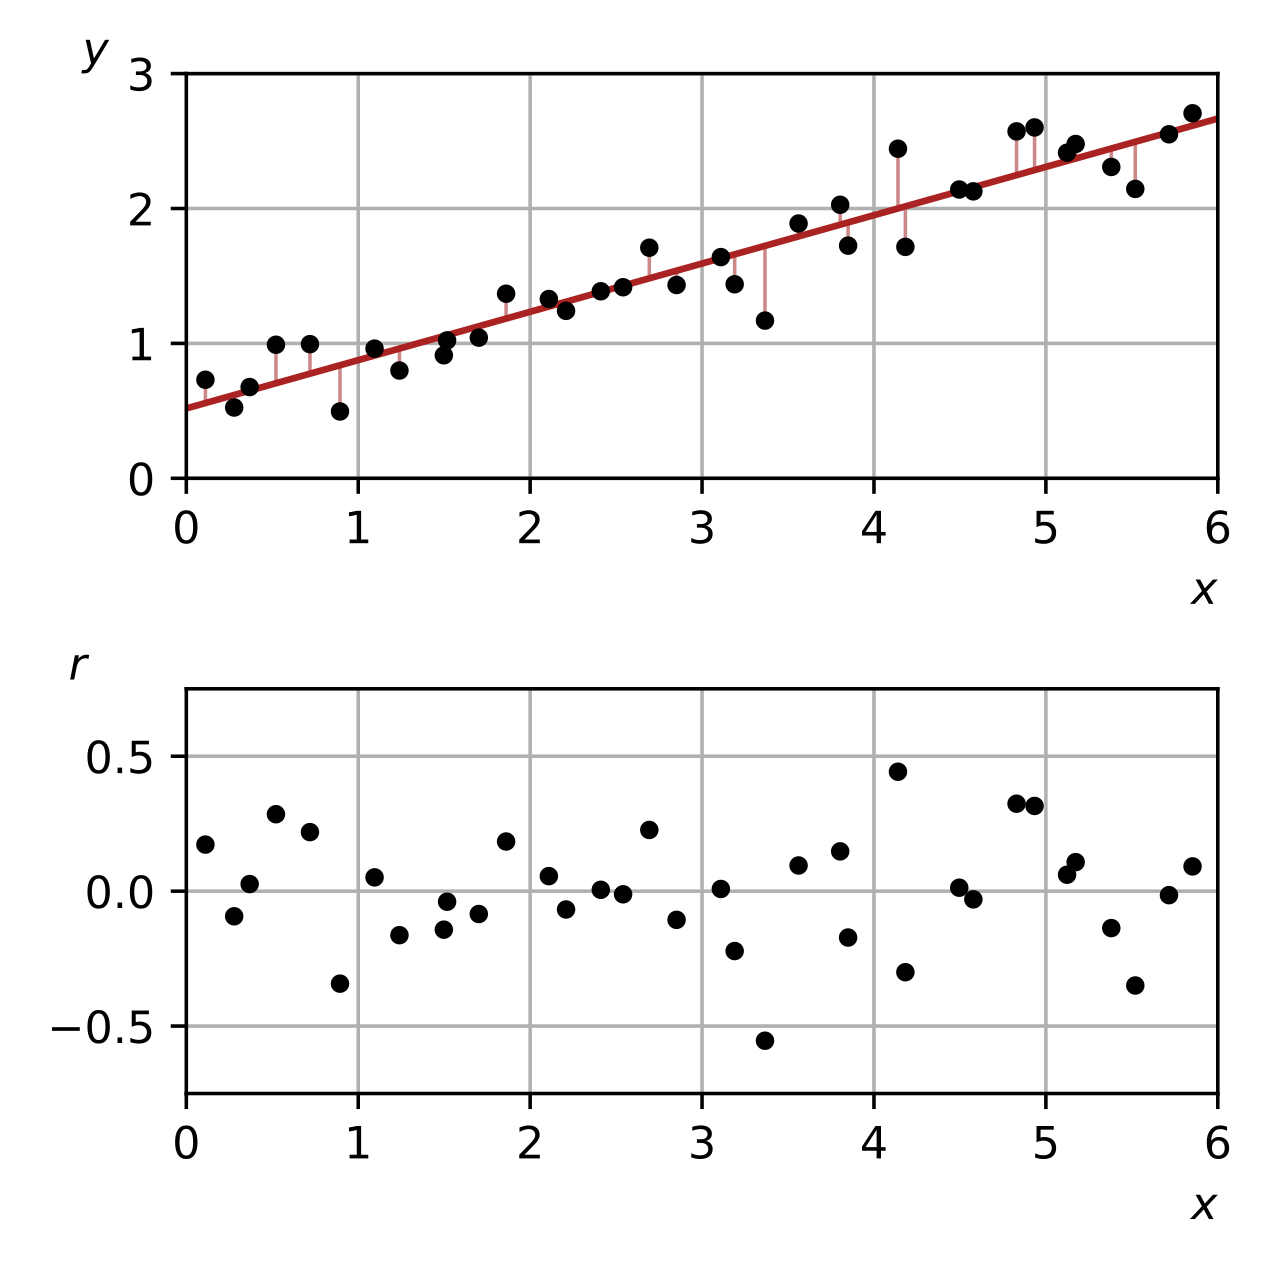
\includegraphics[width=0.78\linewidth]{assets/images/linearni-regrese/linear-regression-residuals.png}
  \caption[Regresní přímka a rezidua]{Regresní přímka a reziduální graf. Popis obrázku: horní panel
  ukazuje body a odhadnutou lineární regresi, dolní panel zobrazuje rezidua vůči vysvětlující proměnné.
  Pokud jsou rezidua náhodně rozptýlená kolem nuly bez systematického vzoru, je lineární specifikace
  věcně přijatelnější. Zdroj obrázku: Justinkunimune,
  \href{https://commons.wikimedia.org/wiki/File:Linear\_regression\_residuals.svg}{Wikimedia Commons},
  licence CC0 1.0.}
  \label{fig:linear-regression-residuals}
\end{figure}

\subsection{Normální rovnice a vlastnosti reziduí}

Z podmínek prvního řádu dostaneme:
\[
X^\top \hat u = 0.
\]

To znamená, že rezidua jsou v odhadnutém modelu nekorelovaná s každou vysvětlující proměnnou zahrnutou
v modelu.

Pokud model obsahuje konstantu, platí také:
\[
\sum_{i=1}^n \hat u_i = 0.
\]

Tedy průměr reziduí je nula.

\subsection{Předpoklady lineárního regresního modelu}

\subsubsection{Linearita v parametrech}

Model je lineární v koeficientech:
\[
y_i = \beta_0+\beta_1x_{i1}+\cdots+\beta_kx_{ik}+u_i.
\]

Proměnné ale mohou být transformované. Model je stále lineární, pokud je lineární v parametrech:
\[
y = \beta_0+\beta_1x+\beta_2x^2+u.
\]

Tento model je lineární v $\beta$, i když vztah mezi $x$ a $y$ je nelineární.

\paragraph{Při porušení.}
Pokud má model špatný funkční tvar, neodpovídá správně podmíněné střední hodnotě
\(\mathrm{E}(y|X)\). OLS potom odhaduje jen nejlepší lineární aproximaci ve vzorku, v reziduích může
zůstávat systematický vzor a koeficienty mohou být vychýlené vůči zamýšlenému efektu, zejména když
chybějící nelineární člen souvisí se zahrnutými regresory. Prakticky se kontrolují reziduální grafy a
podle věcného smyslu se přidávají logaritmy, kvadratické členy, interakce nebo jiné transformace.

\subsubsection{Náhodný výběr}

Pozorování by měla být náhodně vybraná z populace. U průřezových dat se obvykle předpokládá, že jednotky
jsou nezávislé.

\paragraph{Při porušení.}
Pokud vzorek nevznikl náhodně nebo je zatížen selekcí, regresní vztah může popisovat jen dostupný vzorek,
ne cílovou populaci. Jestliže výběr souvisí s nevysvětlenou složkou \(u\), vzniká selection bias a OLS
může být vychýlený. Pokud jsou pozorování závislá, například v klastrech, čase nebo prostoru, samotné
koeficienty nemusí být při exogenitě nutně vychýlené, ale běžné standardní chyby a testy bývají
nespolehlivé. Reakcí jsou výběrové váhy, jasně definovaná cílová populace, klastrované nebo HAC
standardní chyby a modely pro panelová či časová data.

\subsubsection{Žádná perfektní multikolinearita}

Žádná vysvětlující proměnná nesmí být přesnou lineární kombinací ostatních.

\paragraph{Příklad problému.}
Pokud do modelu dáme zároveň všechny dummy proměnné pro kategorie a konstantu, vznikne perfektní
multikolinearita. Proto se jedna kategorie vždy vynechává a slouží jako referenční.

\paragraph{Při porušení.}
Při perfektní multikolinearitě není \(X^\top X\) invertovatelná, takže OLS odhad není jednoznačně
určený. Software typicky některou proměnnou automaticky vyhodí, nebo model vůbec neodhadne. Silná, ale
ne perfektní multikolinearita odhad formálně umožňuje a sama o sobě nezpůsobuje vychýlení, zvyšuje ale
rozptyl odhadů: standardní chyby jsou velké, intervaly spolehlivosti široké a znaménka či velikosti
jednotlivých koeficientů mohou být nestabilní.

\subsubsection{Exogenita}

\[
\mathrm{E}(u|X)=0.
\]

Toto je nejdůležitější předpoklad pro nestrannost a kauzální interpretaci. Znamená, že vysvětlující proměnné
nejsou systematicky spojeny s nepozorovanou složkou $u$.

Porušení exogenity vzniká například při:
\begin{itemize}
    \item vynechané relevantní proměnné,
    \item simultánnosti,
    \item reverzní kauzalitě,
    \item chybě měření ve vysvětlující proměnné.
\end{itemize}

\paragraph{Při porušení.}
OLS je obecně vychýlený a nekonzistentní, takže ani velký vzorek problém automaticky neodstraní.
Koeficient potom směšuje efekt zahrnuté proměnné s vlivem nepozorované složky v chybě a nelze mu dát
kauzální interpretaci. Formálně významný \(t\)-test v takové situaci jen říká, že je odhad přesný kolem
špatného cíle. Typické reakce jsou lepší kontrolní proměnné, proxy proměnné, fixní efekty, instrumentální
proměnné nebo výzkumný design typu difference-in-differences či regression discontinuity.

\subsubsection{Homoskedasticita}

\[
\mathrm{Var}(u|X)=\sigma^2.
\]

Rozptyl chyb je konstantní pro všechny hodnoty $X$.

Pokud rozptyl chyb závisí na $X$, jde o heteroskedasticitu:
\[
\mathrm{Var}(u|X)\neq\sigma^2.
\]

\paragraph{Při porušení.}
Pokud platí exogenita, heteroskedasticita sama o sobě nemusí způsobit vychýlení ani nekonzistenci OLS
koeficientů. Problém je v inferenci: obvyklé standardní chyby, \(t\)-testy, \(F\)-testy, intervaly
spolehlivosti a vlastnost BLUE mohou být špatně. Praktickou reakcí jsou heteroskedasticity-robustní
standardní chyby, vhodná transformace proměnných, vážená metoda nejmenších čtverců nebo lepší
specifikace modelu.

Graficky se často projeví tak, že se rozptyl reziduí systematicky mění s hodnotou vysvětlující proměnné
nebo s predikovanou hodnotou. Typický je \uv{trychtýř}: pro malé hodnoty $x$ jsou rezidua blízko nule,
pro velké hodnoty $x$ se jejich rozptyl zvětšuje.

\begin{figure}[htbp]
  \centering
  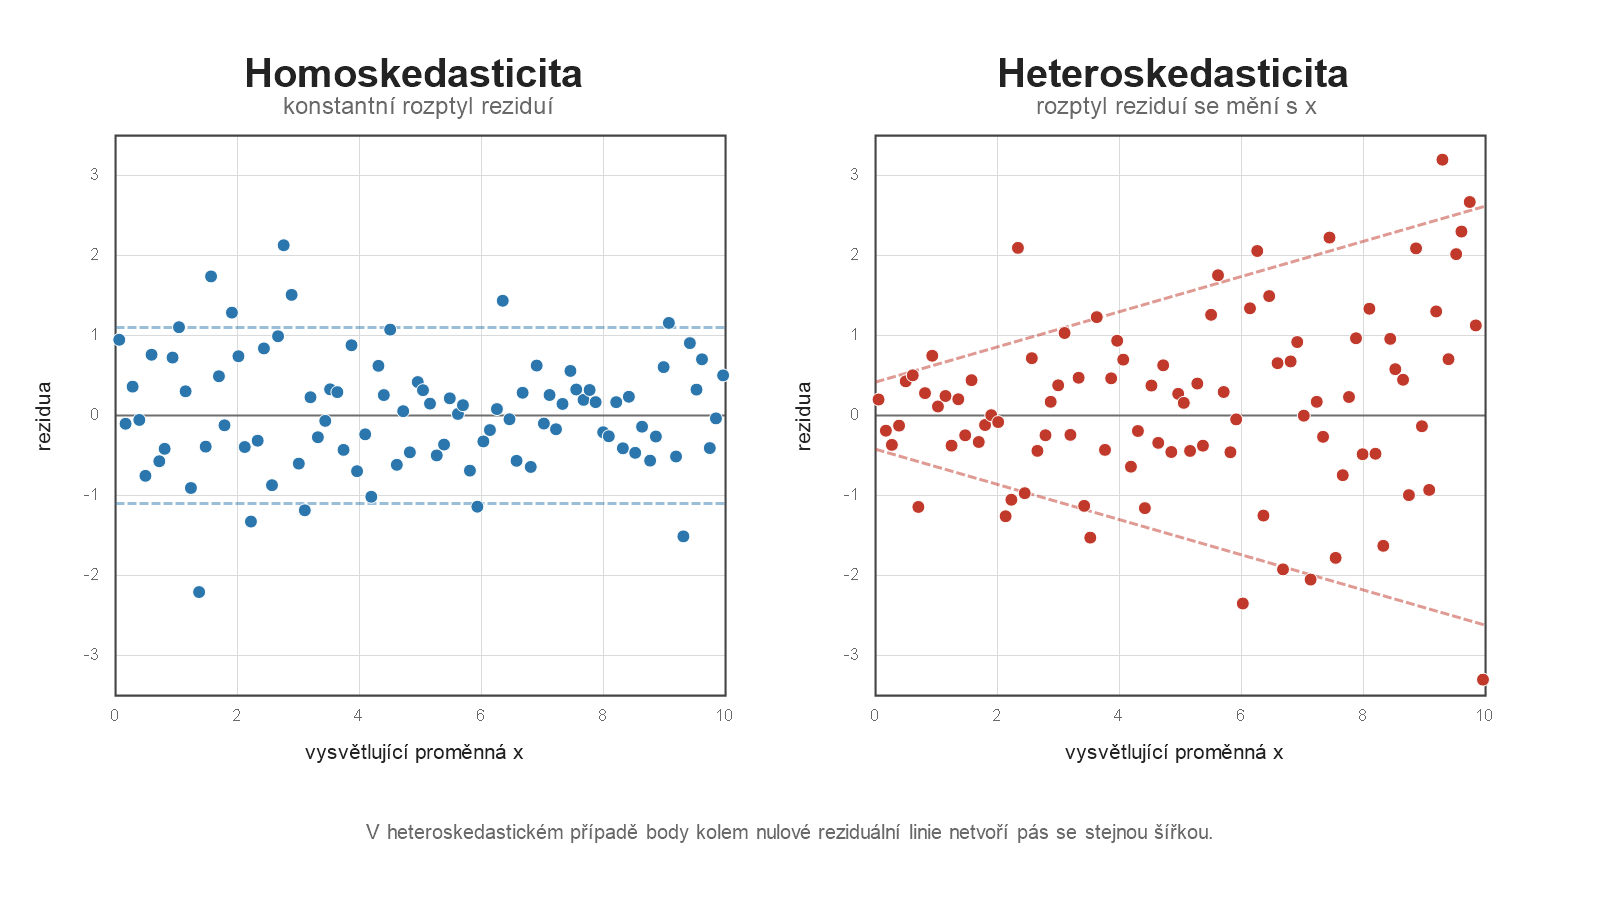
\includegraphics[width=0.95\linewidth]{assets/images/linearni-regrese/homoscedastic-vs-heteroscedastic.png}
  \caption[Homoskedasticita a heteroskedasticita]{Srovnání homoskedasticity a heteroskedasticity v
  reziduálním grafu. Popis obrázku: vlevo mají rezidua přibližně stejný rozptyl pro všechny hodnoty
  $x$, vpravo se rozptyl reziduí s rostoucím $x$ zvětšuje. Zdroj obrázku: vlastní zpracování.}
  \label{fig:homoscedastic-vs-heteroscedastic}
\end{figure}

\subsubsection{Normalita chyb}

\[
u|X \sim N(0,\sigma^2).
\]

Normalita je důležitá hlavně pro přesnou inferenci v malých výběrech. Ve velkých výběrech se často opíráme
o asymptotickou normalitu.

\paragraph{Při porušení.}
Nenormalita chyb sama o sobě nemění vypočtené OLS koeficienty a při splnění ostatních klíčových
předpokladů nebere OLS nestrannost ani konzistenci. V malých vzorcích ale přestávají být přesné klasické
\(t\)-testy, \(F\)-testy, \(p\)-hodnoty a intervaly spolehlivosti odvozené z normality. Ve velkých
vzorcích se používá centrální limitní věta a asymptotická normalita; při těžkých ocasech nebo odlehlých
hodnotách je vhodné zvážit robustní inferenci, bootstrap, transformaci proměnných nebo robustnější
odhadovou metodu.

\paragraph{Zkoušková zkratka.}
LRM.1--LRM.4 jsou klíčové pro nestrannost a konzistenci OLS, LRM.5 přidává obvyklé standardní chyby a
Gaussovu-Markovovu vlastnost BLUE. Normalita chyb není nutná pro velké vzorky, ale dává přesnou
malovýběrovou inferenci.

\subsection{Vlastnosti OLS odhadů}

\subsubsection{Nestrannost}

Pokud platí linearita, náhodný výběr, žádná perfektní multikolinearita a exogenita, potom:
\[
\mathrm{E}(\hat\beta|X)=\beta.
\]

To znamená, že OLS se v průměru trefuje do skutečné hodnoty parametru.

\subsubsection{Konzistence}

Odhad je konzistentní, pokud se s rostoucím počtem pozorování přibližuje ke skutečné hodnotě:
\[
\operatorname{plim}\hat\beta=\beta.
\]

Konzistence je slabší než nestrannost. Odhad může být v malém vzorku vychýlený, ale pokud se s rostoucím
$n$ blíží ke skutečné hodnotě, je konzistentní.

\subsubsection{Rozptyl OLS}

Za homoskedasticity:
\[
\mathrm{Var}(\hat\beta|X)=\sigma^2(X^\top X)^{-1}.
\]

Odhad rozptylu chyb:
\[
\hat\sigma^2 = \frac{SSR}{n-k-1}.
\]

\subsubsection{Gaussova-Markovova věta}

Pokud platí předpoklady LRM včetně homoskedasticity, je OLS:
\[
BLUE = \text{Best Linear Unbiased Estimator}.
\]

To znamená, že mezi lineárními nestrannými odhady má nejmenší rozptyl.

\paragraph{Pozor.}
BLUE neznamená, že OLS je vždy nejlepší možný odhad mezi všemi odhady. Znamená to nejlepší mezi
\emph{lineárními nestrannými} odhady za daných předpokladů.

\subsection{Statistická inference}

Protože pracujeme se vzorkem, odhady se mezi různými vzorky liší. Standardní chyba říká, jak moc je odhad
nejistý:
\[
se(\hat\beta_j).
\]

\subsubsection{t-test jednoho koeficientu}

Testujeme:
\[
H_0:\beta_j=0
\]
proti
\[
H_1:\beta_j\neq 0.
\]

Testová statistika:
\[
t=
\frac{\hat\beta_j-\beta_{j,0}}{se(\hat\beta_j)}.
\]

Nejčastěji:
\[
t=
\frac{\hat\beta_j}{se(\hat\beta_j)}.
\]

Pokud je $|t|$ velké, zamítáme nulovou hypotézu.

Intuice: t-test porovnává \term{velikost odhadu} s \term{nejistotou odhadu}. Koeficient může být věcně
velký, ale pokud má ještě větší standardní chybu, nemáme dost důkazů, že se skutečný populační koeficient
liší od testované hodnoty. Naopak i malý koeficient může být statisticky významný, pokud je odhadnutý
velmi přesně.

\(\beta_{j,0}\) je hodnota koeficientu pod nulovou hypotézou. Nejčastěji testujeme \(\beta_{j,0}=0\),
tedy otázku:
\[
\text{Má proměnná } x_j \text{ při kontrole ostatních proměnných lineární vztah s } y?
\]
Přesněji: test říká, zda je odhadovaný parciální efekt statisticky odlišný od nuly, ne zda je efekt
kauzální, důležitý nebo ekonomicky velký.

Za klasických předpokladů lineárního regresního modelu má testová statistika při platnosti \(H_0\)
t-rozdělení s
\[
n-k-1
\]
stupni volnosti, kde \(n\) je počet pozorování a \(k\) počet vysvětlujících proměnných bez konstanty.
Ve velkých vzorcích se t-rozdělení blíží normálnímu rozdělení, proto se často používá hranice přibližně
\(1.96\) pro oboustranný 5\% test.

\paragraph{p-hodnota.}
p-hodnota říká, jak extrémní t-statistiku bychom dostali, pokud by nulová hypotéza byla pravdivá. Pro
oboustranný test zamítáme \(H_0\) na hladině významnosti \(\alpha\), pokud:
\[
p < \alpha.
\]
Například při \(\alpha=0.05\) zamítáme nulovou hypotézu, pokud je p-hodnota menší než 0.05.

\paragraph{Příklad.}
Odhadneme koeficient u proměnné \(educ\):
\[
\hat\beta_{educ}=1200,
\qquad
se(\hat\beta_{educ})=400.
\]
Test nulové hypotézy \(H_0:\beta_{educ}=0\):
\[
t=\frac{1200-0}{400}=3.
\]
Koeficient je tři standardní chyby od nuly. V běžném velkém vzorku by to znamenalo statisticky významný
výsledek na 5\% hladině. Interpretace ale není \uv{vzdělání určitě kauzálně zvyšuje mzdu o 1200}.
Správnější je: při dané specifikaci modelu je odhadovaný parciální vztah mezi vzděláním a mzdou
statisticky odlišný od nuly.

\paragraph{Pozor na předpoklady.}
Pokud je v modelu heteroskedasticita nebo autokorelace, běžné standardní chyby mohou být špatně odhadnuté
a t-test může zamítat příliš často nebo příliš málo. V takové situaci se obvykle používají robustní
standardní chyby. Pokud je porušena exogenita, t-test může být formálně významný, ale koeficient nemá
čistou kauzální interpretaci.

\subsubsection{Interval spolehlivosti}

\[
\hat\beta_j \pm c \cdot se(\hat\beta_j).
\]

Přibližně pro 95\% interval ve velkém výběru:
\[
\hat\beta_j \pm 1.96 \cdot se(\hat\beta_j).
\]

Interval spolehlivosti ukazuje rozsah hodnot parametru, které jsou s daty a modelem rozumně slučitelné.
U 95\% intervalu neříkáme, že konkrétní interval obsahuje skutečný parametr s pravděpodobností 95\%.
Přesnější interpretace je: kdybychom opakovaně vybírali vzorky a pro každý spočítali interval stejným
postupem, přibližně 95\% takových intervalů by obsahovalo skutečnou hodnotu \(\beta_j\).

Souvislost s t-testem: pokud 95\% interval pro \(\beta_j\) neobsahuje nulu, oboustranný t-test
\(H_0:\beta_j=0\) obvykle zamítne na 5\% hladině. Širší interval znamená větší nejistotu odhadu,
užší interval přesnější odhad.

\subsubsection{F-test více omezení}

Používá se, když testujeme více koeficientů najednou, například:
\[
H_0:\beta_2=\beta_3=\beta_4=0.
\]

F-statistika:
\[
F=
\frac{(SSR_r-SSR_u)/m}{SSR_u/(n-k-1)}.
\]

Kde:
\begin{itemize}
    \item $SSR_r$ je součet čtverců reziduí v restriktivním modelu,
    \item $SSR_u$ je součet čtverců reziduí v neresktriktivním modelu,
    \item $m$ je počet testovaných restrikcí.
\end{itemize}

Restriktivní model vynucuje nulovou hypotézu, například vynechá proměnné \(x_2,x_3,x_4\). Neresktriktivní
model je plný model, kde tyto koeficienty odhadujeme volně. F-test tedy porovnává, jak moc se zhorší fit,
když daná omezení vynutíme.

Intuice: pokud vynechání testovaných proměnných výrazně zvýší reziduální součet čtverců, omezení jsou
pro data nevěrohodná a \(H_0\) zamítáme. F-test je vhodný pro otázky typu \uv{mají tyto proměnné jako
skupina nějaký význam?}. Jednotlivé t-testy by zde nestačily, protože neodpovídají přímo na společnou
hypotézu a zvyšují riziko chyb při opakovaném testování.

\subsection{Dobrota shody}

Celková variabilita:
\[
SST=\sum_{i=1}^n (y_i-\bar y)^2.
\]

\(SST\) měří, jak moc se skutečné hodnoty \(y_i\) celkově liší od svého průměru \(\bar y\). Je to
variabilita, kterou se model snaží vysvětlit.

Nevysvětlená variabilita:
\[
SSR=\sum_{i=1}^n \hat u_i^2.
\]

\(SSR\) zde znamená reziduální součet čtverců, tedy část variability, kterou model nevysvětlil:
\[
\hat u_i = y_i-\hat y_i.
\]
Čím jsou body blíže regresní přímce, tím menší je \(SSR\). V některých učebnicích se stejná veličina
značí \(RSS\) nebo \(SSE\).

U lineární regrese s konstantou platí rozklad:
\[
SST
=
\sum_{i=1}^n(\hat y_i-\bar y)^2
+
\sum_{i=1}^n(y_i-\hat y_i)^2.
\]
Tedy:
\[
\text{celková variabilita}
=
\text{vysvětlená variabilita}
+
\text{nevysvětlená variabilita}.
\]

Koeficient determinace:
\[
R^2=1-\frac{SSR}{SST}.
\]

\(R^2\) říká, jakou část variability \(y\) model vysvětluje. Ekvivalentně:
\[
R^2=
\frac{\text{vysvětlená variabilita}}{\text{celková variabilita}}.
\]
Například pokud \(SST=100\) a \(SSR=25\), potom:
\[
R^2=1-\frac{25}{100}=0.75.
\]
Model tedy vysvětluje 75\% variability \(y\) kolem průměru a 25\% zůstává v reziduích.

\begin{figure}[htbp]
  \centering
  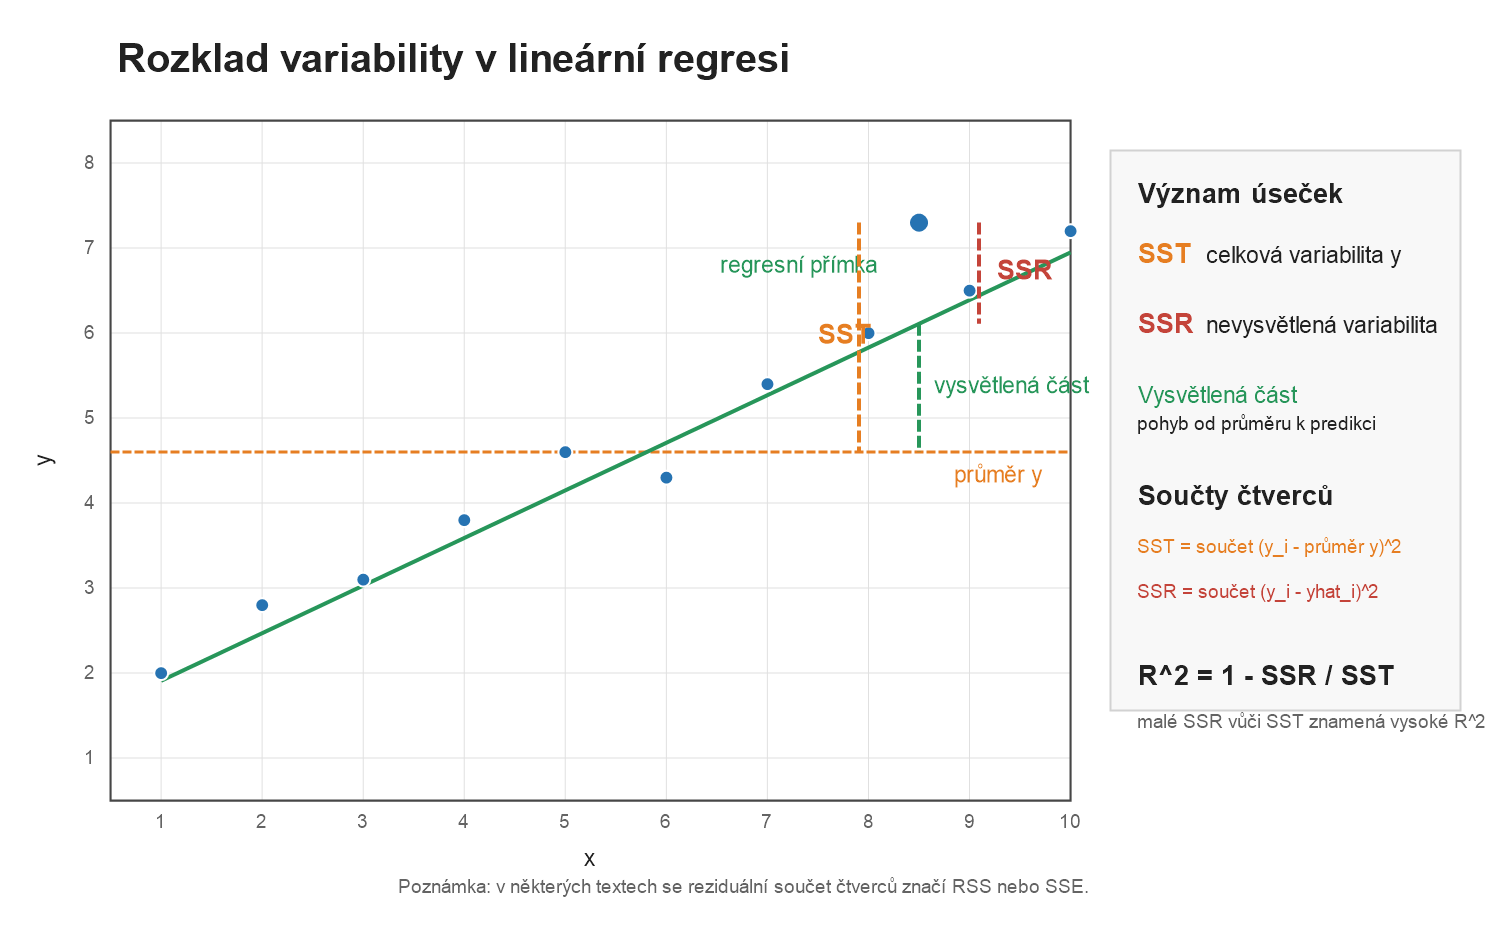
\includegraphics[width=0.95\linewidth]{assets/images/linearni-regrese/r-squared-sst-ssr.png}
  \caption[Rozklad variability v regresi]{Rozklad variability závisle proměnné v lineární regresi.
  Popis obrázku: oranžová úsečka ukazuje celkovou odchylku pozorování od průměru, červená reziduální
  odchylku od regresní přímky a zelená vysvětlenou část mezi průměrem a predikcí. Zdroj obrázku:
  vlastní zpracování.}
  \label{fig:linear-regression-sums-of-squares}
\end{figure}

\paragraph{Pozor.}
Vyšší $R^2$ neznamená automaticky lepší model pro kauzální interpretaci. Model může mít vysoké $R^2$,
ale být špatně specifikovaný nebo trpět endogenitou.

Adjusted $R^2$ penalizuje počet proměnných:
\[
\bar R^2
=
1-
\frac{SSR/(n-k-1)}{SST/(n-1)}.
\]

\subsection{Predikce}

Bodová predikce:
\[
\hat y_0=x_0^\top\hat\beta.
\]

Je důležité rozlišovat dva typy nejistoty:

\begin{itemize}
    \item interval spolehlivosti pro průměrnou hodnotu $\mathrm{E}(y|x_0)$,
    \item predikční interval pro konkrétní nové pozorování $y_0$.
\end{itemize}

Predikční interval je širší, protože obsahuje:
\begin{itemize}
    \item nejistotu v odhadu regresní funkce,
    \item náhodnou individuální odchylku $u$.
\end{itemize}

Přibližně:
\[
\hat y_0
\pm
c
\sqrt{
x_0^\top \widehat{\mathrm{Var}}(\hat\beta)x_0
+
\hat\sigma^2
}.
\]

\begin{figure}[htbp]
  \centering
  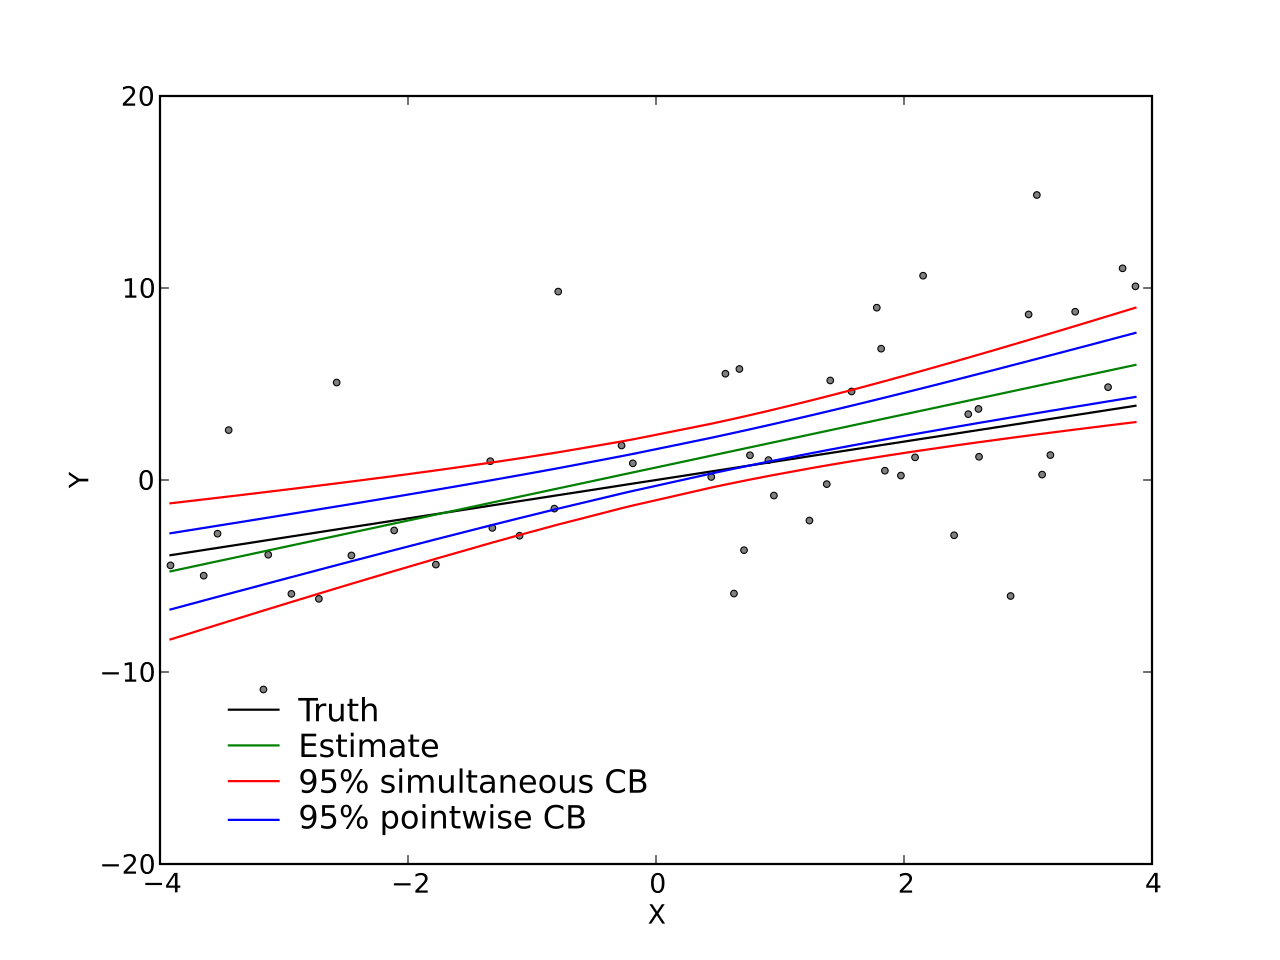
\includegraphics[width=0.82\linewidth]{assets/images/linearni-regrese/regression-confidence-band.png}
  \caption[Regresní nejistota]{Odhadnutá regresní funkce a pásy nejistoty. Popis obrázku: zelená
  křivka je odhad, modré a červené pásy ukazují různé typy konfidenčních pásem kolem regresní funkce.
  Pásy se typicky rozšiřují dál od středu dat, kde je odhad méně opřený o pozorování. Zdroj obrázku:
  Skbkekas, \href{https://commons.wikimedia.org/wiki/File:Regression\_confidence\_band.svg}{Wikimedia Commons},
  licence CC BY 3.0.}
  \label{fig:regression-confidence-band}
\end{figure}

\paragraph{Extrapolace.}
Regrese predikuje nejspolehlivěji v oblasti hodnot, které jsou podobné trénovacím datům. Predikce mimo
pozorovaný rozsah $x$ je extrapolace a může být zavádějící i tehdy, když má model v trénovacích datech
vysoké $R^2$.

\subsection{Volba modelu}

Při volbě modelu řešíme:
\begin{itemize}
    \item které proměnné zahrnout,
    \item jak je transformovat,
    \item zda zahrnout interakce,
    \item zda vztah není nelineární,
    \item zda model slouží k popisu, predikci nebo kauzalitě.
\end{itemize}

\subsubsection{Volba podle účelu}

\begin{itemize}
    \item \textbf{Deskriptivní model} má přehledně popsat vztahy v datech. Důležitá je srozumitelná
    interpretace koeficientů a transparentní specifikace.
    \item \textbf{Prediktivní model} vybíráme podle chyby na validačních nebo testovacích datech.
    Může obsahovat proměnné, které zlepšují predikci, i když nemají čistou kauzální interpretaci.
    \item \textbf{Kauzální model} stavíme kolem identifikační otázky. Klíčové je zahrnout relevantní
    confoundery, vyhnout se špatným kontrolním proměnným a obhájit exogenitu.
\end{itemize}

Proto neexistuje jeden univerzálně \uv{nejlepší} regresní model. Model s nejvyšším $R^2$ nemusí být
nejlepší pro predikci mimo trénovací data a už vůbec nemusí identifikovat kauzální efekt.

\subsubsection{Křížová validace, informační kritéria a regularizace}
U prediktivních úloh se model volí podle výkonu mimo trénovací data. \term{Holdout} rozdělí data na
trénovací, validační a testovací část. \term{k-fold cross-validation} rozdělí data na \(k\) částí,
model vždy trénuje na \(k-1\) částech a testuje na zbývající části; výsledná chyba je průměr přes
všechny foldy. Testovací množina se používá až na konečné nezávislé vyhodnocení.

\term{AIC} a \term{BIC} porovnávají modely pomocí věrohodnosti penalizované za počet parametrů.
Nižší hodnota znamená lepší kompromis mezi shodou s daty a složitostí. AIC obvykle penalizuje
složitost mírněji, BIC přísněji, protože penalizace roste s velikostí vzorku. U lineární regrese se
často sleduje také adjustované \(R^2\), které na rozdíl od běžného \(R^2\) trestá zbytečné proměnné.

\term{Ridge} regrese používá \(L_2\) penalizaci:
\[
  \min_\beta \sum_{i=1}^n (y_i-x_i^\top\beta)^2 + \lambda \sum_{j=1}^p \beta_j^2.
\]
Koeficienty zmenšuje směrem k nule, ale obvykle je nenastaví přesně na nulu. Hodí se při multikolinearitě
a v situacích, kdy mnoho proměnných nese malou část signálu.

\term{LASSO} používá \(L_1\) penalizaci:
\[
  \min_\beta \sum_{i=1}^n (y_i-x_i^\top\beta)^2 + \lambda \sum_{j=1}^p |\beta_j|.
\]
Může některé koeficienty nastavit přesně na nulu, takže funguje jako výběr proměnných. Pokud jsou ale
prediktory silně korelované, může vybrat jen jeden z několika podobných prediktorů.

\term{Elastic net} kombinuje \(L_1\) a \(L_2\) penalizaci. Prakticky je užitečný, když chceme zároveň
stabilizovat odhady a provádět výběr proměnných.

U všech penalizovaných regresí je zásadní \term{škálování prediktorů}. Penalizace působí na velikost
koeficientů, takže proměnná měřená v korunách, tisících korun nebo procentech by bez standardizace
dostala jiný trest. Proto se numerické prediktory typicky standardizují a parametr \(\lambda\) se volí
pomocí validačních dat nebo křížové validace. Intercept se obvykle nepenalizuje.

\subsubsection{Dummy proměnné}

Kategoriální proměnné se do regrese dávají pomocí dummy proměnných.

Pokud má proměnná tři kategorie, například:
\[
\text{Felicia, Octavia, Superb},
\]
vložíme do modelu jen dvě dummy proměnné. Jedna kategorie je referenční.

Příklad:
\[
price = \beta_0+\beta_1 km+\beta_2 year+\beta_3 Octavia+\beta_4 Superb+u.
\]

Pokud je referenční kategorie Felicia, potom:
\begin{itemize}
    \item $\beta_3$ říká, o kolik se liší Octavia od Felicie při stejném $km$ a $year$,
    \item $\beta_4$ říká, o kolik se liší Superb od Felicie při stejném $km$ a $year$.
\end{itemize}

\subsubsection{Logaritmické transformace}

Model:
\[
\log(y)=\beta_0+\beta_1x+u.
\]

Interpretace:
\[
100\beta_1
\]
je přibližná procentní změna $y$ při jednotkové změně $x$.

Přesná procentní změna:
\[
100(e^{\beta_1}-1).
\]

Model:
\[
\log(y)=\beta_0+\beta_1\log(x)+u.
\]

Zde je $\beta_1$ elasticita:
\[
1\% \text{ změna } x
\quad \Rightarrow \quad
\beta_1\% \text{ změna } y.
\]

\paragraph{Logaritmus a kvantilové kódování.}
Logaritmus je pro kladné hodnoty monotónní transformace. Nemění pořadí pozorování, takže pokud se
kategorie tvoří jen podle kvantilů téže proměnné, stejné jednotky zůstanou ve stejných kvantilových
skupinách. Změní se ale vzdálenosti mezi hodnotami a interpretace rozdílů, což může být důležité pro
regresi nebo metody citlivé na měřítko.

\subsubsection{Kvadratický člen}

Pokud vztah není lineární, můžeme přidat $x^2$:
\[
y=\beta_0+\beta_1x+\beta_2x^2+u.
\]

Marginální efekt:
\[
\frac{\partial \mathrm{E}(y|x)}{\partial x}
=
\beta_1+2\beta_2x.
\]

Bod obratu:
\[
x^*=-\frac{\beta_1}{2\beta_2}.
\]

\subsubsection{Interakce}

Interakce znamená, že efekt jedné proměnné závisí na hodnotě jiné proměnné:
\[
y=\beta_0+\beta_1x+\beta_2z+\beta_3xz+u.
\]

Efekt $x$:
\[
\frac{\partial \mathrm{E}(y|x,z)}{\partial x}
=
\beta_1+\beta_3z.
\]

\paragraph{Příklad.}
Efekt vzdělání na mzdu se může lišit podle pohlaví. Potom do modelu přidáme interakci:
\[
wage=\beta_0+\beta_1educ+\beta_2female+\beta_3(educ\cdot female)+u.
\]

\subsection{Vynechaná proměnná a omitted variable bias}

Skutečný model:
\[
y=\beta_0+\beta_1x+\gamma z+u.
\]

Pokud ale odhadneme model bez $z$:
\[
y=\alpha_0+\alpha_1x+v,
\]
může vzniknout vychýlení.

Vzorec pro omitted variable bias:
\[
\operatorname{plim}(\tilde\beta_1)
=
\beta_1
+
\gamma\frac{\mathrm{Cov}(x,z)}{\mathrm{Var}(x)}.
\]

Bias vzniká, pokud platí obě podmínky:
\begin{itemize}
    \item $z$ ovlivňuje $y$, tedy $\gamma\neq 0$,
    \item $z$ koreluje s $x$, tedy $\mathrm{Cov}(x,z)\neq 0$.
\end{itemize}

\paragraph{Intuice.}
Pokud vynechaná proměnná souvisí s vysvětlující proměnnou, model její efekt mylně přičte proměnné $x$.

Možné reakce závisí na povaze problému. \term{Proxy proměnná} je pozorovatelná náhrada nepozorovaného
faktoru, například testové skóre jako přibližná kontrola schopností v regresi mzdy na vzdělání.
Proxy se vkládá přímo do rovnice a pomáhá snížit vychýlení, pokud dobře zachycuje vynechaný faktor.
\term{Instrumentální proměnná} se používá, když je vysvětlující proměnná endogenní. Dobrý instrument
musí být relevantní pro endogenní proměnnou a zároveň exogenní vůči chybě v hlavní rovnici. Častým
odhadem je dvoustupňová metoda nejmenších čtverců, zkráceně 2SLS.

\subsection{Multikolinearita}

Multikolinearita znamená, že vysvětlující proměnné jsou mezi sebou silně korelované.

Rozptyl koeficientu:
\[
\mathrm{Var}(\hat\beta_j)
=
\frac{\sigma^2}{SST_j(1-R_j^2)}.
\]

Kde:
\begin{itemize}
    \item $SST_j$ je variabilita proměnné $x_j$,
    \item $R_j^2$ je $R^2$ z pomocné regrese $x_j$ na ostatní vysvětlující proměnné.
\end{itemize}

Variance Inflation Factor:
\[
VIF_j=\frac{1}{1-R_j^2}.
\]

Vysoký $VIF$ znamená, že $x_j$ je silně vysvětlitelná ostatními regresory.

\paragraph{Důsledek.}
Multikolinearita obvykle nezpůsobuje vychýlení, ale zvyšuje standardní chyby. Koeficienty jsou pak
nepřesné, intervaly spolehlivosti široké a proměnné mohou vycházet statisticky nevýznamné.

\subsection{Heteroskedasticita}

Heteroskedasticita:
\[
\mathrm{Var}(u_i|X_i)\neq \sigma^2.
\]

Typicky se objevuje například u příjmových dat, kde lidé s vyšším příjmem mají často větší variabilitu.

\paragraph{Důsledek.}
Pokud platí exogenita, OLS koeficienty mohou být stále nestranné a konzistentní. Problém je ve standardních
chybách:
\[
se(\hat\beta_j)
\]
mohou být špatně odhadnuté.

Řešení:
\begin{itemize}
    \item heteroskedasticity-robust standard errors,
    \item vážené nejmenší čtverce,
    \item vhodná transformace proměnných.
\end{itemize}

\begin{figure}[htbp]
  \centering
  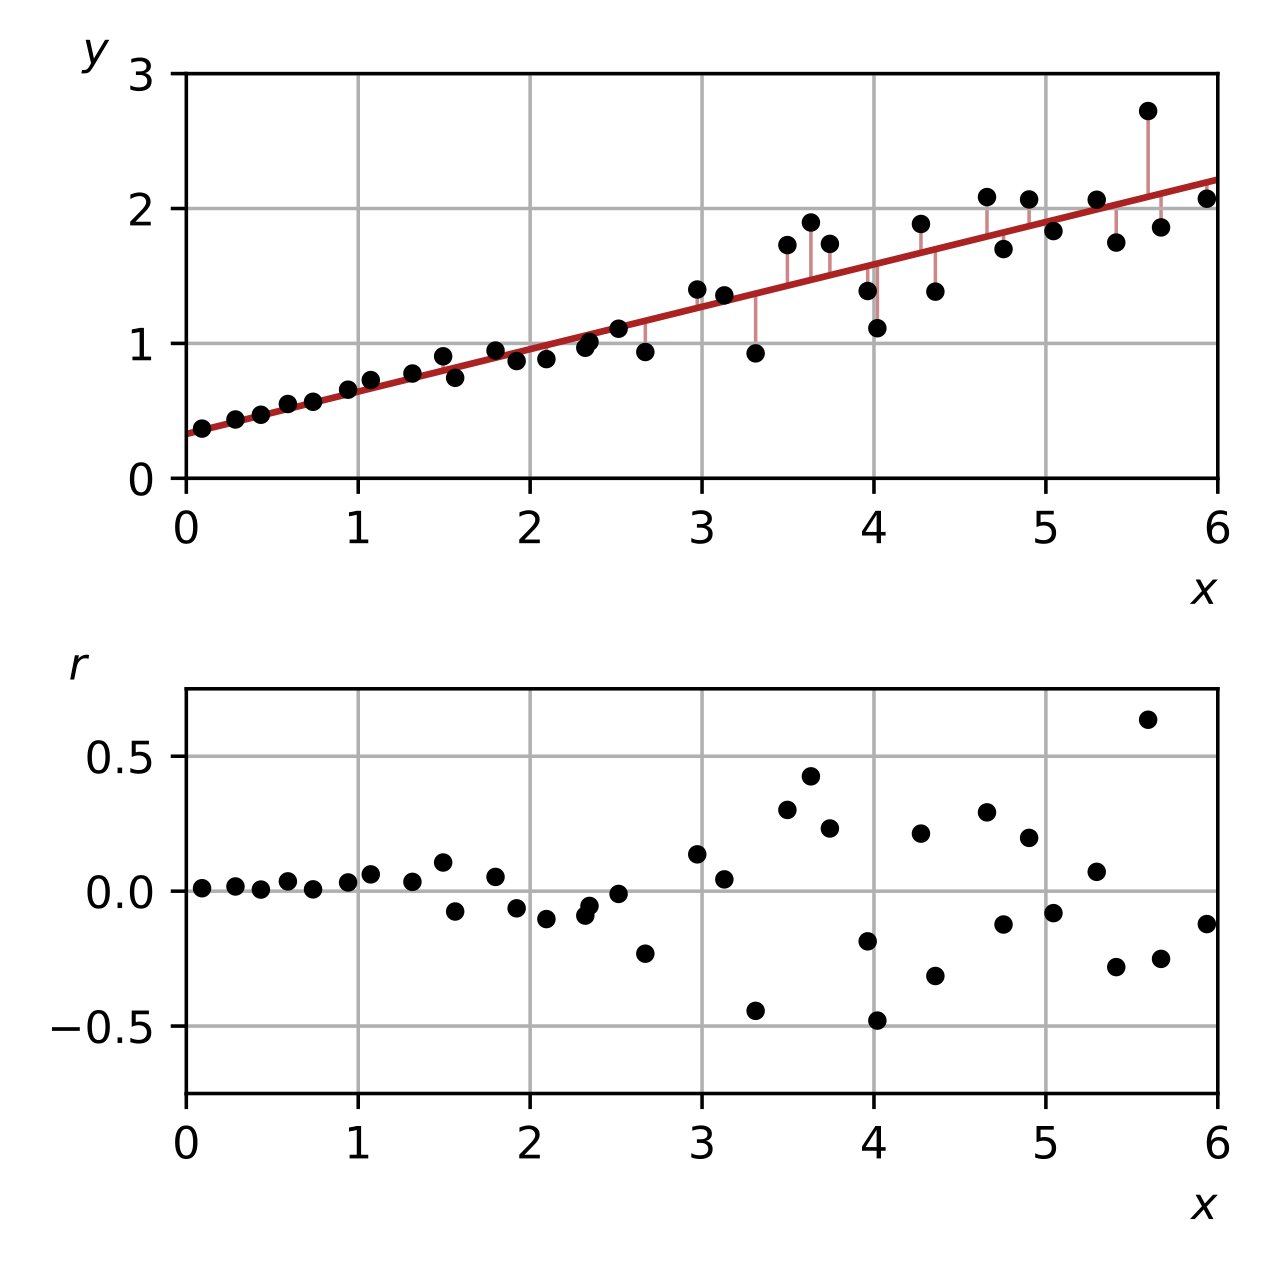
\includegraphics[width=0.78\linewidth]{assets/images/linearni-regrese/heteroscedastic-residuals.png}
  \caption[Heteroskedasticita v reziduích]{Reziduální graf s heteroskedasticitou. Popis obrázku:
  horní panel ukazuje lineární regresi, dolní panel ukazuje, že rozptyl reziduí není konstantní, ale
  roste s hodnotou vysvětlující proměnné. V takové situaci je potřeba řešit zejména správné
  standardní chyby a inferenci. Zdroj obrázku: Justinkunimune,
  \href{https://commons.wikimedia.org/wiki/File:Linear\_regression\_residuals\_heteroscedastic.svg}{Wikimedia Commons},
  licence CC0 1.0.}
  \label{fig:heteroscedastic-residuals}
\end{figure}

\subsection{Diagnostika regresního modelu}

Po odhadu nestačí opsat tabulku koeficientů. Je potřeba ověřit, zda model odpovídá účelu analýzy.

Typicky kontrolujeme:
\begin{itemize}
    \item \textbf{rezidua vs. fitted values} -- vzor v reziduích může znamenat nelinearitu,
    heteroskedasticitu nebo chybějící proměnné;
    \item \textbf{odlehlá a vlivná pozorování} -- extrémy mohou výrazně změnit koeficienty;
    \item \textbf{multikolinearitu} -- vysoké VIF a široké intervaly spolehlivosti u klíčových
    proměnných;
    \item \textbf{normalitu reziduí} -- hlavně pro malovýběrovou inferenci;
    \item \textbf{predikční výkon} -- u prediktivních úloh validační/testovací chyba, například RMSE
    nebo MAE;
    \item \textbf{věcnou plausibilitu} -- znaménka, velikosti efektů a jednotky musejí dávat ekonomický
    smysl.
\end{itemize}

\subsection{Pozor u zkoušky}

Nejčastější chyba je zaměnit statistickou významnost za věcnou nebo kauzální významnost. Malé
$p$-value říká, že odhad je vzhledem ke standardní chybě vzdálený od nulové hypotézy, ne že efekt je
velký, důležitý nebo kauzální. Druhá častá chyba je tvrdit, že vysoké $R^2$ znamená správný model.
Pro kauzalitu je důležitá exogenita a argument o tom, proč v chybě nezůstává confounder. Pro predikci je
důležitá chyba na nových datech, ne jen fit v trénovacím souboru.

\subsection{Shrnutí ke zkoušce}

Lineární regrese modeluje podmíněnou střední hodnotu $y$ pomocí lineární kombinace vysvětlujících
proměnných. OLS minimalizuje součet čtverců reziduí:
\[
\hat\beta=(X^\top X)^{-1}X^\top y.
\]
Regrese může sloužit k deskripci, predikci i kauzální analýze, ale kauzální interpretace vyžaduje především
exogenitu:
\[
\mathrm{E}(u|X)=0.
\]
Při splnění základních předpokladů je OLS nestranný a konzistentní; při homoskedasticitě je BLUE.
Při praktickém použití je nutné řešit volbu modelu, vynechané proměnné, multikolinearitu,
heteroskedasticitu a správnou interpretaci koeficientů.

\subsection{Zdroje}
\begin{itemize}
    \item statsmodels User Guide:
    \href{https://www.statsmodels.org/stable/regression.html}{Linear Regression}.
    \item scikit-learn User Guide:
    \href{https://scikit-learn.org/stable/modules/linear\_model.html}{Linear Models}.
    \item PennState Eberly College of Science:
    \href{https://online.stat.psu.edu/stat501/}{STAT 501 -- Regression Methods}.
    \item Zeileis:
    \href{https://cran.r-project.org/web/packages/sandwich/vignettes/sandwich.pdf}{Econometric Computing with HC and HAC Covariance Matrix Estimators}.
    \item Wikimedia Commons:
    \href{https://commons.wikimedia.org/wiki/File:Linear\_regression\_residuals.svg}{File:Linear\_regression\_residuals.svg}.
    \item Wikimedia Commons:
    \href{https://commons.wikimedia.org/wiki/File:Linear\_Regression\_Plot.png}{File:Linear\_Regression\_Plot.png}.
    \item Wikimedia Commons:
    \href{https://commons.wikimedia.org/wiki/File:Regression\_confidence\_band.svg}{File:Regression\_confidence\_band.svg}.
    \item Wikimedia Commons:
    \href{https://commons.wikimedia.org/wiki/File:Linear\_regression\_residuals\_heteroscedastic.svg}{heteroskedastic residual plot}.
\end{itemize}

\newpage
